\documentclass[zihao=-4]{ctexart}
\usepackage{xeCJKfntef}
\usepackage[paperwidth=10cm,paperheight=16cm,textwidth=240bp,vmargin=0.5cm]{geometry}
\pagestyle{empty}
% \usepackage[a4paper,textwidth=492bp,vmargin=2cm]{geometry}

\usepackage{mwe}
\usepackage{amssymb,amsmath}
\usepackage{unicode-math}
\usepackage{siunitx}

\setmainfont{Fira Sans}
\setmathfont{Fira Math}
% \setmainfont{XITS}
% \setmathfont{XITS Math}
\xeCJKsetup{PunctStyle=kaiming}
\setCJKmainfont[Mapping=fullwidth-stop]{Source Han Sans CN}
% \setCJKmainfont[Mapping=fullwidth-stop]{Source Han Serif CN}
\setCJKsansfont{Source Han Sans CN}
\RequirePackage{enumitem,calc}
\setlist[enumerate,1]{leftmargin=0pt,labelsep=0pt,itemindent=0pt,parsep=5pt,itemsep=0pt,topsep=0pt,partopsep=0pt,listparindent=2\ccwd}
\setlist[enumerate,2]{leftmargin=0pt,labelsep=0pt,itemindent=1\ccwd+0.17cm,parsep=5pt,itemsep=0pt,topsep=0pt,partopsep=0pt,listparindent=2\ccwd}
\def\labelenumi{\theenumi、}
\def\labelenumii{(\theenumii)}

\def\xiahua#1{\CJKunderline[hidden=false,thickness=1pt]{#1}}
\let\siold\si
\let\SIold\SI
\renewcommand{\si}[1]{\mbox{\siold{#1}}}
\renewcommand{\SI}[2]{\mbox{\SIold{#1}{#2}}}
\makeatletter
\def\@maketitle{%
  \newpage
  \null
  \vskip 2em%
  \begin{center}%
  \let \footnote \thanks
    {\LARGE \@title \par}%
  \end{center}%
  \par
  \vskip 1.5em}
\makeatother
\title{《新能源与微电网技术》复习题}

\begin{document}
\maketitle
\section{填空题}
\begin{enumerate}
\item \xiahua{储能技术}是指将\xiahua{电力能量}转变成其他形式的\xiahua{储存}于一种介质之中,并在需要的时候把这些能量以\xiahua{电能}的形式释放出来的技术。
\item \xiahua{抽水蓄能电站}是目前在实际工程中技术最成熟,同时应用最为广泛的一种储能方式。
\item \xiahua{压缩空气储能电站}实质上是一种用于调峰的燃气轮机发电厂。
\item 飞轮储能装置主要由\xiahua{高速飞轮}、\xiahua{电动机}、轴承支撑系统、\xiahua{电子控制系统}和真空泵、\xiahua{功率变换器}、紧急备用轴承等设备组成。
\item 超级电容器由2个\xiahua{多孔电极}、\xiahua{隔膜}以及\xiahua{电解质}组成,它是根据电化学双电层理论研制而成的,因此又称为\xiahua{双电层电容器},其具有比普通电容器更强的储电能力。
\item 抽水蓄能电站在建造容量方面具有很大的灵活性,能量利用效率在\xiahua{ $\SI{70}{\percent} \sim \SI{85}{\percent}$}。
\item 分布式电源对电压分布的影响主要取决于\xiahua{分布式电源的容量}、接入位置和功率因数。
\item 微电网是由\xiahua{分布式发电},储能装置,用电负荷、监控、保护和自动化装置等组成,能够实现内部电力自主平衡的小型供电网络。
\item 微电网的主体供电线路采用直流供电方式的叫\xiahua{直流微电网}。
\item 微电网并网运行时,一旦与其连接的\xiahua{配电网的电压}或\xiahua{频率}出现异常,且异常持续时间超出了微电网内负荷所允许的范围,则微电网将由并网运行转为离网运行。
\item 太阳能电池的类型多种多样,目前发展最成熟的是\xiahua{硅太阳能电池},其在应用中居主导地位。目前光伏系统的投资大约为\xiahua{ 2.2 万元/\si{kW}},而太阳能光伏发电成本约为\xiahua{ 2 元/\si{kWh}}。
\item 微电网本体成本主要指微电网及分布式电源项目\xiahua{本体规划}、建设、\xiahua{调试}等引发的成本,可分为直接成本和间接成本,直接成本主要包括\xiahua{设备采购}、\xiahua{施工调试}、\xiahua{土地建设}等费用,间接成本包括\xiahua{咨询设计}、\xiahua{项目审批}、税费等部分。
\item 常见的、比较受到关注的分布式发电技术有\xiahua{风力发电技术}、太阳能光伏发电技术、\xiahua{微型燃气发电技术}和\xiahua{燃料电池发电技术}等。
\item 光伏系统应用非常广泛,其基本发电模式可以分为两大类:\xiahua{独立发电}系统和\xiahua{并网发电系统}。
\item 分布式电源的接入使配电系统从放射形无源网络变为遍布负荷和中小型电源的有源网络,这将对系统的\xiahua{潮流分布}、继电保护、网络损耗、\xiahua{电能质量}、电网可靠性以及\xiahua{电网调度}产生重要影响,甚至威胁电力系统的安全运行。
\item CCHP以\xiahua{天然气}为主要燃料,也可使用\xiahua{煤气}、沼气或油气等其他可燃气体。
\item 以\xiahua{动能}和势能的形式储存电能的机械储,如抽水蓄能(pumped hydropower plant,PHPP)、\xiahua{压缩空气}储能(compressed air energy storage,CAES)、飞轮储能(flywheel energy storage,FWES)等。
\end{enumerate}

\section{解释名词}
\begin{enumerate}
\item 光伏发电:光伏发电是将太阳能直接转换为电能的一种发电形式。
\item 智能优化算法:适用于多目标优化问题的智能优化算法不再单纯地从纯数学的推导演
化中寻求 Pareto 最优解,而是借鉴于生命科学与信息科学的发展而形成的交叉领域中衍生
而来。智能优化算法通过模拟生物进化以及群体动物活动等生命特征,运用迭代计算实现对
多目标优化问题的求解。
\item 微电网:微电网是分布式发电的重要形式之一,它是指将一定区域内分散的
小型发电单元组织起来形成一个微型网络为本区域的当地负荷供冷、热和电或与
传统电网并联。
\item 风力发电:风力发电区别于传统发电模式的最大特点是:风能是随机的,风
向和风速都是随时随机变化的,因其输入的不确定性导致功率输出的不确定性。
\item 电池储能:电池储能利用电池正负极的氧化还原反应进行充放电工作。
\item 优化算法:将多目标优化问题通过一定的人为方法将其转化为单目标优化问
题,然后求解转化后的单目标优化问题。
\item 双向变流器:是实现电池储能系统与外部交流系统双向能量互动的装置。
\item 冷热电联供:是一种将热机、发电机、热回收和制冷装置作为整体,通过统
一管理制冷供热及供电过程。
\item 最大功率点跟踪:在光伏发电系统中,要提高系统的整体效率,一个重要的
途径就是实时检测光伏阵列的输出功率,通过一定的控制算法预测当前工况下阵
列可能的最大功率输出,从而改变当前的阻抗情况,调整光伏阵列的工作点,使
之始终工作在最大功率点附近,这一过程就称之为最大功率点跟踪(maximum
power point tracking, MPPT)。
\item 光伏电池:光伏电池的基本结构是一个半导体二极管,有光照时,光伏电池
的输出特性类似于一个二极管,电流随电压成指数变化。
\item 低压微电网:是目前实验室和商业工程中应用最为广泛的微电网模式。可以
作为微电网的一个最小单元集群。
\item Agent:是指由一系列数据库、软件、硬件组成的,能够完成某一特定功能的
集合。
\item MPPT:在光伏发电系统中,要提高系统的整体效率,一个重要的
途径就是实时检测光伏阵列的输出功率,通过一定的控制算法预测当前工况下阵
列可能的最大功率输出,从而改变当前的阻抗情况,调整光伏阵列的工作点,使
之始终工作在最大功率点附近,这一过程就称之为最大功率点跟踪(maximum
power point tracking, MPPT)。
\end{enumerate}


\section{简答题}
\begin{enumerate}
\item 阻容模型中,蓄电池组被看成为由两个电容和四个电阻所构成的混联等效电路,请同学简单绘制出阻容模型等效电路,并说明电路中各个参数。

\newcommand{\xiabiao}[2]{#1_\mathrm{#2}}
\noindent 答:等效电路见图~\ref{fig:1}。

$U_{\mathrm{DC}}$ 为蓄电池组的开路电压;$I_{\mathrm{L2}}$ 为电池组电流;$C_{\mathrm{b}}$ 与 $r_{\mathrm{b}}$ 并联,用以体现蓄电
池组的自放电情况;$r_{\mathrm{bs}}$ 为蓄电池组的连接电阻;$\xiabiao{r}{bt}$ 为蓄电池组内阻;$\xiabiao{C}{bp}$ 和 $\xiabiao{r}{bp}$ 并联,用以体现蓄电池组的超电动势。
\begin{figure}[!htbp]
  \centering
  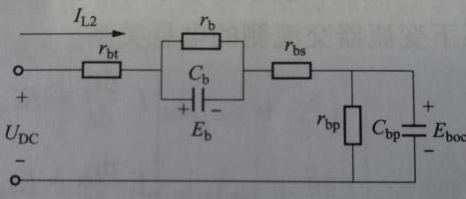
\includegraphics[width=0.5\textwidth]{fig1.png}
  \caption{阻容模型等效电路}\label{fig:1}
\end{figure}
\item 微电网对电网的影响和灵活性方面提出的“即插即用”指的是什么?

\noindent 答:(网络答案)
\begin{enumerate}
  \item 当大电网中存在多个微电网的时候,微电网对大电网能够即插即用;
  \item 微电网内部的不同分布式电源对微电网能够即插即用。
\end{enumerate}
\item 微电网的能量优化的优化算法有那些请详细说明?

\noindent 答:主要有:图解法、数学优化算法、多目标优化算法。
\begin{enumerate}
  \item 图解法: 图解法一般指基于长时间尺度的光照和风速数据,使用图解法来得到最优电
  源出力和蓄电池容量组合的方法。该方法优化过程考虑较少的变量,一 般只考虑两个变量,
  如光伏电池和蓄电池容量,或者光伏电池和风机容量,因此得出的优化结果具有一定的片面
  性。
  \item 数学优化算法:微电网优化模型中存在着各种约束,网络约束为非线性约束,而考虑分
  布式发电的开停机状态会使得模型中存在整数变量等。
  \item 多目标优化算法:在微电网优化运行时,往往需要综合若干种子目标进行综合评估,因
  此需要建立相应的多目标优化模型,采用多目标优化算法综合分析。
\end{enumerate}
\item 什么是中压交流微电网?

\noindent 答: 中压交流微电网适用于分布式电源容量较大、渗透率高,并且需要保证供电可靠性的
敏感负荷分布不集中的场合,其特点是 \SI{10}{kV} 中压馈线上含有容量较大的分布式电源,(如集
中型的风电场和光伏电站),而在低压配电二次侧也分布着一定数量的低压微电网或者小容
量的分布式电源,其中每个子微电网可以独立构成一个供能系统。
\item 请详细说明压缩空气储能电站主要原理?且绘制出压缩空气储能电站结构示意图。
\begin{figure}[!htbp]
  \centering
  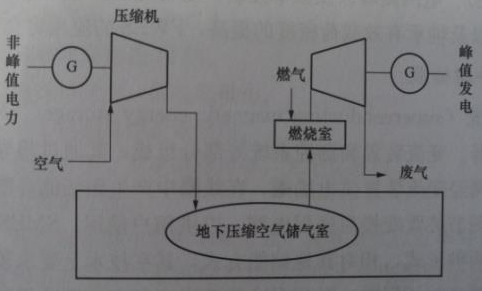
\includegraphics[width=0.5\textwidth]{fig2.png}%
  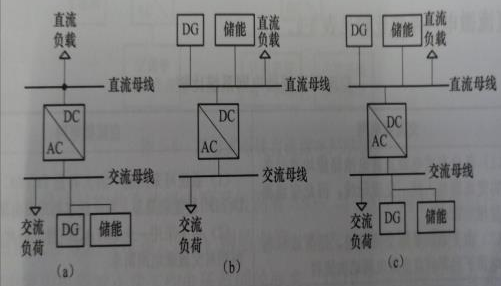
\includegraphics[width=0.5\textwidth]{fig3.png}
  \caption{压缩空气储能电站结构示意图}\label{fig:2}
\end{figure}

\noindent 答:
压缩空气储能电站(compressed air energy storage, CAES) 实质上是一种用于调峰的燃气
轮机发电厂,其主要原理利用电力系统负荷低谷时段的剩余电力进行压缩空气作业,并将其
储存于高压密封设施内,在负荷高峰时段释放出来用以驱动燃气轮机发电。在 CAES 发电过
程中,所消耗的燃气量要比常规燃气轮机少 \SI{40}{\percent},能量利用效率得到了较大提升,同时在节
约成本方面也很有优势。CAES 主要在实际中的用途主要是峰谷电能回收调节、频率调制、
平衡负荷、分布式储能以及发电系统备用,其优点是 CAES 储气库安全性比较高,运行可靠,
寿命长,能够适用于冷启动、黑启动等,且响应速度快。

示意图见图~\ref{fig:2}。

\item 画出各类交直流微电网典型结构模式图?

\noindent 答:交直流微电网典型结构模式图见图~\ref{fig:3}。

\begin{figure}[!htbp]
  \centering
  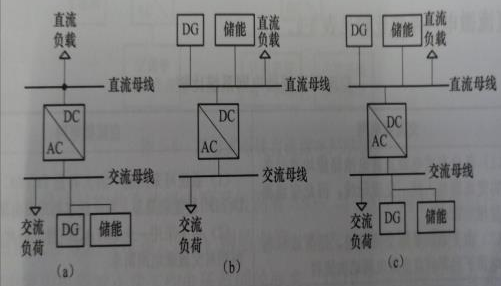
\includegraphics[width=0.5\textwidth]{fig3.png}
  \caption{交直流微电网各类典型结构模式。(a)第一类;(b)第二类;(c)第三类}\label{fig:3}
\end{figure}

\item 请同学简单绘制出光伏电池模型等效电路,并说明电路中各个参数。

\noindent 答:等效电路见图~\ref{fig:4}。

$I$ 为光伏电池输出电流;$\xiabiao{I}{ph}$ 为光生电流;$\xiabiao{I}{D}$ 为光伏电池反向饱和电流;$\xiabiao{R}{sh}$ 为
并联等效电阻;$\xiabiao{I}{sh}$ 为流经 $\xiabiao{R}{sh}$ 电流;$\xiabiao{R}{s}$ 为串联等效电阻;$U$ 为光伏电池输出电压;$\xiabiao{R}{L}$ 为等效负载。

\begin{figure}[!htbp]
  \centering
  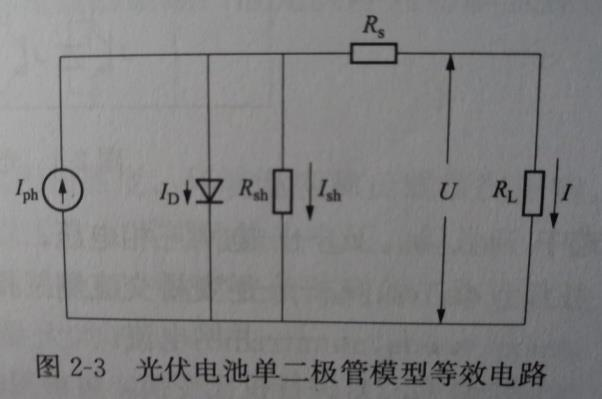
\includegraphics[width=0.5\textwidth]{fig4.png}
  \caption{光伏电池单二极管模型等效电路}\label{fig:4}
\end{figure}

\item 什么是孤岛效应?孤岛效应有哪些危害?

\noindent 答:(书本寻找)当电网供电因故障、事故或停电维修而跳开时,接入各用户端
的分布式电源可能和周围的负载构成自给供电的孤岛,即所谓的孤岛效应。

当分布式电源切换成孤岛方式运行时,如果没有储能元件或其容量太小,就会容易导致
电压波动与闪变。对于单相光伏电池,当其脱离原有的配电网后,原来的单相供电模式可能
造成其他配电网内出现三相负载不对称的情形,还有可能影响到其他用户的电压质量。

(网络答案) 孤岛效应是指并入公共电网中的发电装置,在电网断电的情况下,
这个发电装置却不能检测到或根本没有相应检测手段,仍然向公共电网馈送电量
的现象。

孤岛效应的危害有:
\begin{enumerate}
  \item 危害电力维修人员的生命安全;
  \item 影响配电系统上的保护开关动作程序;
  \item 孤岛区域所发生的供电电压与频率的不稳定性质会对用电设备带来破坏;
  \item 当供电恢复时造成的电压相位不同步将会产生浪涌电流,可能会引起再
  次跳闸或对发电系统、负载和供电系统带来损坏;
  \item 并网发电系统因单相供电而造成系统三相负载的缺相问题。
\end{enumerate}
\end{enumerate}
\section{选择题、是非题}
没给。
\section{附录}
吴寅:「附记:仅个人意见,部分题目书中提供有不同答案,网络提供也有差异,可
按各自意见更改。」
\end{document}
